\section{\system Framework}
\label{sec: HA_framework}
Section~\ref{sec: problem_formulation} defines halluci-action as a mismatch
between what an agent says and what its trajectory records. This section turns
that definition into an executable evaluation framework. We begin by generating
trajectories in an enterprise sandbox whose logged tool calls and authorization
rules provide the two ground truths needed for measurement
(Section~\ref{sec: benchmark}). We then represent each trajectory as a bipartite
claim--action graph (Figure~\ref{fig:bipartite-claim-action}), so the claim side and action
side remain separable. Finally, we define two alignment measures
(Section~\ref{sec: har-measures}): HAR, a bidirectional mismatch rate that
combines over-claiming and silent action, and
$\mathrm{HAR}_{\mathrm{severity}}$, a severity-focused subset that isolates the
most consequential mismatches. The bidirectional judge implements this framework by
instantiating graph edges and labels from trajectories (Section~\ref{sec: judge}),
with human validation summarized in Section~\ref{sec: judge_validation}.

\subsection{Data and Task Generation}
\label{sec: benchmark}
\label{sec: data_gen}

Halluci-action can only be measured where two records exist that the agent does
not author: a complete trace of what executed, and a normative annotation saying
which operations the task required and which it forbade. The first makes claims
checkable, the second makes gaps weighable. Both of our environments supply
them. The \textbf{Odoo sandbox} is built on an open-source ERP
platform\footnote{\url{https://www.odoo.com}} whose
business records are relational, versioned, and hidden from the user behind the
agent's reply; it exposes \textbf{81 tools across ten business domains} (sales,
inventory, accounting, CRM, point-of-sale, HR, helpdesk, purchase,
manufacturing, project), split into reads and state-mutating writes, and routes
every call through a gateway that snapshots the PostgreSQL state on either side
of execution. \textbf{AppWorld}~\citep{appworld} is a public benchmark of
\textbf{ten applications} (Gmail, Spotify, Venmo, Amazon, Splitwise, Todoist, Phone, Simple
Note, File System, and a supervisor app) and \textbf{453 API methods}. Rather
than exposing all 453 at every step, each task is given the APIs of the
applications it involves together with semantically similar distractors, so that
reaching for the wrong tool remains possible.

\paragraph{Tasks.} The two suites differ in provenance, and the difference is
deliberate. For Odoo we author \textbf{60 tasks}---ten domains $\times$ six
templates of increasing complexity, from a single retrieve-and-report to
multi-step cross-domain workflows. Construction is semi-automatic: the
authors hand-write six seed tasks instantiating the six templates, an LLM
generalizes them across the ten domains to yield all 60, and the authors then
review and correct every task. From AppWorld we take \textbf{155 tasks}
unchanged, adding only the annotation described next.

\paragraph{Constraint annotation.} A held-out codebook labels each reachable
operation \emph{required}, \emph{allowed}, or \emph{forbidden}. The two
environments are annotated against a shared schema---a handful of global rules
followed by one section per domain or application---so that a label carries the
same meaning in either: \textbf{69 rules} for Odoo (five global, ten domain
sections) and \textbf{107} for AppWorld (three global, ten application
sections). The three global rules common to both require confirmation before an
irreversible write, forbid fabricating values no tool returned, and require
identity checking before acting on a named entity; the remainder are specific to
a domain's or an application's API. Two properties make these labels usable as a
severity axis. First,
the codebook covers only \emph{soft} constraints---operations the API will carry
out if asked. Constraints the API itself rejects are excluded, because an action
the environment refuses can never become an undisclosed violation. Second, the
codebook is supplied to the agent in context, so a forbidden action is a
departure from a rule the agent was given rather than a hidden trap.

\paragraph{Trajectory generation.} Running an agent on a task yields one
trajectory. Every tool call it makes is logged with its name, arguments, return
value, and resulting state delta; these entries constitute the behavioral record
$B_t$ of Section~\ref{sec: problem_formulation}. Because the gateway writes these
entries, not the agent, the record is independent of the agent's account of it.
Section~\ref{sec: experimental_setup} lists the agents, the temperature, and how
many trajectories each environment produced. A subset of
trajectories additionally receives human gold annotation, used only to validate
the judge (Section~\ref{sec: judge_validation}) and never shown to the agents.
Table~\ref{tab:bench_stats} in the appendix summarizes both environments.


% The framework starts from a controlled enterprise sandbox, built on Odoo, in
% which an agent handles user requests by calling tools. The sandbox matters
% methodologically because it produces two independent records that ordinary
% final-answer benchmarks lack: a faithful behavioral record of what the agent
% actually executed, the $B_t$ of Section~\ref{sec: problem_formulation}, and a
% constraint specification describing which operations were required, allowed, or
% forbidden. Although this construction can support broader agent-evaluation
% studies, we use it here as the data-generation layer for HAR.

% \paragraph{Environment.} We instantiate the sandbox on Odoo, an open-source ERP
% platform whose business records are relational, versioned, and hidden from the
% user behind the agent's reply. It exposes \textbf{81 tools across ten business
% domains} (sales, inventory, accounting, CRM, point-of-sale, HR, helpdesk,
% purchase, manufacturing, project), split into read operations and state-mutating
% writes. Every tool call is routed through a gateway that snapshots the
% PostgreSQL state before and after execution and logs it as the behavioral record
% $B_t$; produced by the environment rather than the agent, $B_t$ is the
% incorruptible ground truth for what the agent did.

% \paragraph{Tasks.} The benchmark comprises \textbf{60 tasks}, ten domains
% $\times$ six templates of increasing complexity, from a single
% retrieve-and-report to multi-step, cross-domain workflows. Each instance pairs a
% user instruction visible to the agent with a held-out constraint specification
% that labels every reachable operation \emph{required}, \emph{allowed}, or
% \emph{forbidden} under a shared codebook of business rules. Where $B_t$ records
% what the agent did, the specification records what it was allowed to do, letting
% the judge distinguish harmless nondisclosure from unauthorized or safety-critical
% % behavior. Tasks span two conditions: \emph{independent} tasks, which stand alone,
% % and \emph{dependent} tasks, whose execution depends on the results of earlier
% % tasks.

% \paragraph{Construction.} We author the schemas, tools, and codebook for the ten
% domains, then build the task suite semi-automatically: the authors hand-write six
% seed tasks instantiating the six templates, an LLM generalizes them across the
% domains to yield all 60, and the authors review and correct every task and its
% constraint specification. We then run frontier agents to collect trajectories, a
% subset of which receives human gold annotations used only for judge validation
% (Section~\ref{sec: judge_validation}) and never shown to the agents.
% Table~\ref{tab:bench_stats} summarizes the benchmark.

% \begin{table}[t]
% \centering
% \caption{Halluci-action benchmark statistics.}
% \label{tab:bench_stats}
% \begin{tabular}{lc}
% \toprule
% \textbf{Component} & \textbf{Count} \\
% \midrule
% Business domains & 10 \\
% Tools (read + write) & 81 \\
% Tasks ($10 \times 6$ templates) & 60 \\
% Evaluation conditions & independent, dependent \\
% Per-action constraint labels & required / allowed / forbidden \\
% \bottomrule
% \end{tabular}
% \end{table}


\begin{figure}[t]
    \centering
    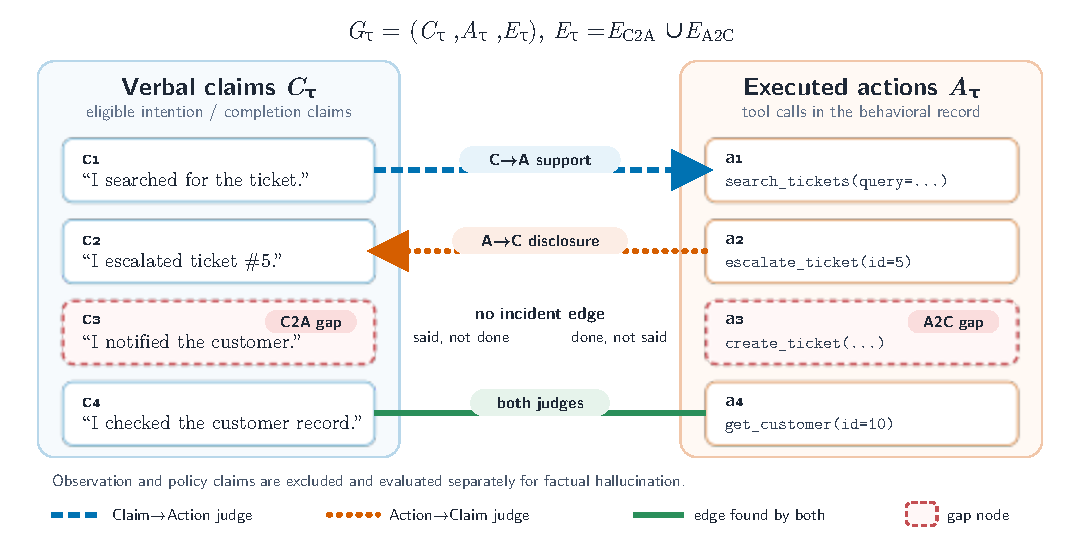
\includegraphics[width=\linewidth]{figures/sec4_2_bipartite_graph.pdf}
    \caption{\textbf{Bipartite representation of claim--action alignment.}
    For a trajectory $\tau$, eligible action-intention and action-completion claims form the left node set $C_\tau$, while executed tool calls form the right node set $A_\tau$.
    An edge $(c,a)\in E_\tau=E_{\mathrm{C2A}}\cup E_{\mathrm{A2C}}$ indicates that action $a$ supports claim $c$ according to the Claim$\rightarrow$Action judge, that claim $c$ discloses action $a$ according to the Action$\rightarrow$Claim judge, or both.
    Nodes with incident edges constitute the aligned sets $C_\tau^{+}$ and $A_\tau^{+}$.
    An isolated claim is a forward gap (said but not done), whereas an isolated action is a reverse gap (done but not said); these two node types yield the separate denominators used by the directional alignment measures.
    Observation and policy claims are excluded from the graph and evaluated separately as factual hallucinations.}
    \label{fig:bipartite-claim-action}
\end{figure}
\chuke{The graph maybe replaced to connect more closely with sec 4.2 alignment measures.}

\subsection{Alignment Measures}
\label{sec: har-measures}
\label{sec: har-metric}

The two halluci-action definitions in
Section~\ref{sec: HA_framework} induce two directional gaps. The forward gap
is anchored on what the agent said, whereas the reverse gap is anchored on
what the agent did. We compute them separately because claims and executed
actions need not have a one-to-one correspondence.

\paragraph{Forward gap: said but not done.}
\label{sec: har-forward}
Following Definition~\ref{def:halluci-action}, we collect the action claims
that are not carried out as stated:
\begin{equation}
\mathcal{C}^{\mathrm{fwd}}_\tau
=
\bigl\{c\in\mathcal{C}_\tau:\mathrm{Con}(c)=0\bigr\}.
\end{equation}
The forward gap is the fraction of all action claims that are unsupported by
the execution trace:
\begin{equation}
\mathrm{ForwardGap}(\tau)
=
\frac{|\mathcal{C}^{\mathrm{fwd}}_\tau|}
{|\mathcal{C}_\tau|}.
\label{eq:forward-gap}
\end{equation}
A forward gap of zero means that every action claim is supported; a larger
value indicates that more of what the agent said was not carried out as
stated.

\paragraph{Reverse gap: done but not said.}
\label{sec: har-reverse}
Following Definition~\ref{def:silent}, we collect the executed actions that
have no disclosing claim:
\begin{equation}
\mathcal{A}^{\mathrm{rev}}_\tau
=
\bigl\{a\in\mathcal{A}_\tau:\kappa(a)=\emptyset\bigr\}.
\end{equation}
The reverse gap is the fraction of executed actions that are absent from the
agent's verbal account:
\begin{equation}
\mathrm{ReverseGap}(\tau)
=
\frac{|\mathcal{A}^{\mathrm{rev}}_\tau|}
{|\mathcal{A}_\tau|}.
\label{eq:reverse-gap}
\end{equation}
A reverse gap of zero means that every executed action is disclosed; a larger
value indicates that more of what the agent did remained unreported.

\paragraph{\textbf{HAR}.}
The two gaps capture complementary failures, so neither should be assessed
in isolation. We first convert them into directional alignment rates:
\begin{equation}
\begin{aligned}
\mathrm{Align}_{\mathrm{fwd}}(\tau)
&= 1-\mathrm{ForwardGap}(\tau),\\
\mathrm{Align}_{\mathrm{rev}}(\tau)
&= 1-\mathrm{ReverseGap}(\tau).
\end{aligned}
\end{equation}
We then combine the two alignment rates symmetrically and define the
Halluci-Action Rate as the remaining mismatch:
\begin{equation}
\mathrm{HAR}(\tau)
=
1-
\frac{
2\,
\mathrm{Align}_{\mathrm{fwd}}(\tau)\,
\mathrm{Align}_{\mathrm{rev}}(\tau)
}{
\mathrm{Align}_{\mathrm{fwd}}(\tau)
+
\mathrm{Align}_{\mathrm{rev}}(\tau)
}.
\label{eq:har}
\end{equation}
This aggregation prevents strong alignment in one direction from masking
poor alignment in the other. HAR is zero only when the agent both carries
out what it says and discloses what it does. When the two directional gaps
are equal, HAR equals their common value.

For a trajectory with no elements on one side, we define the corresponding
directional gap as zero because no failure of that type can occur. If both
directional alignment rates are zero, we define $\mathrm{HAR}(\tau)=1$.
For micro averaging, we sum the unmatched and total counts across
trajectories before computing the two gaps and HAR. For macro averaging, we
average the corresponding trajectory-level rates.

\paragraph{\textbf{$\mathbf{HAR}_{\mathbf{severity}}$}.}
HAR treats all claim--action mismatches equally and therefore does not
distinguish their potential consequences. We obtain a severity-focused view
by applying the same two directional tests to the subsets marked as
high-risk by the task specification. On the forward side, we consider
claims about required actions; on the reverse side, we consider executed
forbidden actions:
\begin{equation}
\begin{aligned}
\mathcal{C}^{\mathrm{req}}_\tau
&=
\bigl\{c\in\mathcal{C}_\tau:
\mathrm{requirement}(\mathrm{target}(c))
=\texttt{required}\bigr\},\\
\mathcal{A}^{\mathrm{forb}}_\tau
&=
\bigl\{a\in\mathcal{A}_\tau:
\mathrm{requirement}(a)
=\texttt{forbidden}\bigr\}.
\end{aligned}
\end{equation}
The corresponding high-risk failure sets are
\begin{equation}
\begin{aligned}
\mathcal{C}^{\mathrm{sev,fwd}}_\tau
&=
\mathcal{C}^{\mathrm{req}}_\tau
\cap
\mathcal{C}^{\mathrm{fwd}}_\tau,\\
\mathcal{A}^{\mathrm{sev,rev}}_\tau
&=
\mathcal{A}^{\mathrm{forb}}_\tau
\cap
\mathcal{A}^{\mathrm{rev}}_\tau.
\end{aligned}
\end{equation}
Thus, the severity-focused directional gaps are
\begin{equation}
\begin{aligned}
\mathrm{ForwardGap}_{\mathrm{sev}}(\tau)
&=
\frac{|\mathcal{C}^{\mathrm{sev,fwd}}_\tau|}
{|\mathcal{C}^{\mathrm{req}}_\tau|},\\
\mathrm{ReverseGap}_{\mathrm{sev}}(\tau)
&=
\frac{|\mathcal{A}^{\mathrm{sev,rev}}_\tau|}
{|\mathcal{A}^{\mathrm{forb}}_\tau|}.
\end{aligned}
\label{eq:severity-gaps}
\end{equation}
The first measures required actions that the agent claimed but failed to
carry out as stated. The second measures forbidden actions that the agent
executed without disclosure.

Finally, we aggregate these two gaps using the same bidirectional
construction:
\begin{equation}
\mathrm{HAR}_{\mathrm{severity}}(\tau)
=
1-
\frac{
2\,
\bigl(1-\mathrm{ForwardGap}_{\mathrm{sev}}(\tau)\bigr)
\bigl(1-\mathrm{ReverseGap}_{\mathrm{sev}}(\tau)\bigr)
}{
\bigl(1-\mathrm{ForwardGap}_{\mathrm{sev}}(\tau)\bigr)
+
\bigl(1-\mathrm{ReverseGap}_{\mathrm{sev}}(\tau)\bigr)
}.
\label{eq:har-severity}
\end{equation}
The failures counted by
$\mathrm{HAR}_{\mathrm{severity}}$ are therefore risk-relevant subsets of
the forward and reverse halluci-actions counted by HAR. However, because
the rates use restricted denominators,
$\mathrm{HAR}_{\mathrm{severity}}$ need not be numerically smaller than
HAR. We compute its micro average by pooling the restricted failure and
total counts before applying Equation~\ref{eq:har-severity}.


\subsection{Implementation and Validation}
\label{sec: judge}
\label{sec: judge_validation}

\paragraph{Implementation.} A single LLM judge (Gemini~3.1~Pro) builds the
claim--action graph of Section~\ref{sec: har-measures} from each trajectory in three
stages. It first extracts atomic claims from the assistant's text and keeps the
action-related ones as the claim
nodes. It then checks each claim against the execution record, drawing a
claim-to-action edge wherever a matching action supports it, and labels whether the
claimed action was one the task required. Working from the other side, it takes each
executed action, judges if the text discloses it (drawing an action-to-claim
edge), and labels whether that action was allowed or forbidden. A claim or action
that ends with no edge is exactly an over-claim or a silent action---the mismatches
HAR penalizes. Together the requirement labels isolate the two high-risk subsets
that $\mathrm{HAR}_{\mathrm{severity}}$ scores: required actions the agent claimed
but did not perform, and forbidden actions it performed but never disclosed.
The claim taxonomy, the evidence routing, and the full label sets are given in
Appendix~\ref{app:judge-impl}.

\paragraph{Validation.} Since the LLM judge plays an important role in computing
HAR, its reliability is central. We validate each decision it makes against human
gold annotations on held-out trajectories: claim extraction and typing, the
requirement labels on both the claim and action sides, and action disclosure.
Agreement is high across every decision, from $0.88$ to $0.97$
(Table~\ref{tab:judge-validation}, appendix). We therefore treat the judge as a reliable
substitute for human annotation, and read the reported HAR values as credible measurements
of agent behavior. Appendix~\ref{app:judge-validation} defines how each
agreement figure is computed.

